\chapter{Introduction}~\label{chap:intro}

The aim of this thesis is to demonstrate the viability of the digital back-end novel of a novel pixelated readout to be used in Time Projection Chambers (TPCs). 
We begin this chapter with an introduction to the Standard Model (SM) in Section~\ref{sec:standard_model}.
We pay particular attention to the experimental work which was done to lay the foundation of the knowledge of physics we have today.

In Section~\ref{sec:tpcs} we briefly discuss the history and development TPCs. 
The novel readout presented in this thesis is in Chapter~\ref{chap:qpix} is designed specifically for use in TPC detectors.
Chapter~\ref{chap:saq} provides the first measurements Q-Pix front-end readout in gas-based TPCs.

We continue in Section~\ref{sec:dune} to describe the future Deep Underground Neutrino Experiment (DUNE).
The studies of Chapters~\ref{chap:qdb} and~\ref{chap:sim} demonstrate how this novel charge readout could be scaled to a DUNE Far Detector (DUNE-FD) scale.

In Section~\ref{sec:neutrino_oscillation} we provide a brief history on the discovery of the neutrino and discuss its relevance for searching for physics beyond the Standard Model.
We also provide a short review of the theory behind neutrino oscillations.
Oscillation measurements, and by extension, the search for Charge-Parity violation in the lepton sector are primary science goals of the DUNE experiment.
These measurements involve interactions which occur at~\unit{GeV} energy scales.
We provide the first demonstration of required capabilities at these energy scales for the Q-Pix back-end readout in Chapter~\ref{chap:sim}.

Finally, we finish this chapter on a discussion on the developments of new tracking detectors and highlight their relevance to the work presented here.

\section{The State of Things: The Standard Model}~\label{sec:standard_model}

What is the universe made of?
What are the fundamental building blocks of matter?
Since time immemorial thinkers have questioned the nature of the universe and wondered what the basic building blocks of nature are.
The answer to these fundamental questions is the motivation for particle physics.

In the history of science, it is easy to argue that the most successful of all models is the Standard Model of Physics.
The Standard Model (SM)~\citep{GLASHOW1961579, salam1964electromagnetic, weinberg1967model} was originally developed in the mid to late 1970's and is the model responsible for unifying the weak, strong, and electromagnetic forces together.
It has made remarkable predictions about the existence of elusive neutrinos, quarks and vector bosons before their discovery, and more.

The comprehensive and extensive list of known particles, as well as various cross-sections, lifetimes, and other known information can be found from the bi-annually published Particle Data Group (PDG)~\citep{Workman:2022ynf}.
The SM has been experimentally tested more exhaustively any other theory.
The SM has stood the test of time, despite the many mysteries it can not explain.

\subsection{The Basics of the Standard Model}

The SM itself dictates the fundamental constituents of matter and energy.
Its purpose is to explain the origin of observed matter as well as provide a description of all observable interactions.
The interactions described by the SM involve three of the four known fundamental forces observed in nature: the electromagnetic, weak, and strong forces.
The missing fourth force is one of the major shortcomings of the SM: its inability to incorporate a quantum description of gravity.

All currently known fundamental particles are represented in Fig.~\ref{fig:cern_sm}.
These particles represent the today's knowledge of the building blocks of all observed matter in the universe.

\begin{figure}[]
\centering
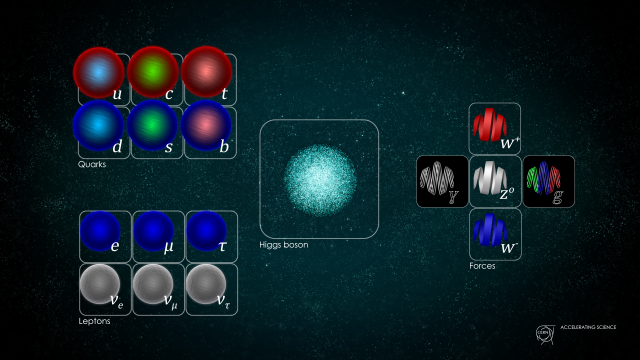
\includegraphics[width=\textwidth]{images/STDM_higgs_and_field_D.png}
\caption{Image of fundamental particles in the Standard Model, taken from~\citep{dominguez_2015}.
  All known matter and particle interactions involves combinations of the particles shown here.}
\label{fig:cern_sm}
\end{figure}


The quarks represent particles in the top left of Figure~\ref{fig:cern_sm}.
In 1961 Murray Gell-Mann proposed his ``eight-fold way''~\citep{eightfold_way_osti_4008239}, which provided a method of grouping the hadrons.
Following shortly later, the quark model was then propossed by Gell-Mann in 1964~\citep{quark_model_GELLMANN1964214}.
A unique feature of quarks compared to leptons is that no ``free'' quark has ever been observed.
This means that all current direct observations of quarks are in bound states.

\begin{table}
\begin{center}
\begin{tabular}{||c c c c c||}
 \hline
 Quark & Charge & Mass (MeV) & Year Discovered & Ref.\\ [0.5ex]
 \hline\hline
 up & $\frac{2}{3}$ & 2.16 & 1968 & SLAC~\citep{1969PhRvL..23..930B, 1969PhRvL..23..935B} \\
 \hline
 down & $\frac{-1}{3}$ & 4.67 & 1968 & SLAC~\citep{1969PhRvL..23..930B, 1969PhRvL..23..935B} \\
 \hline
 strange & $\frac{-1}{3}$ & 93.4 & 1968 & SLAC~\citep{1969PhRvL..23..930B, 1969PhRvL..23..935B} \\
 \hline
 charm & $\frac{2}{3}$ & 1270 & 1974 & SLAC~\citep{augustin1974observation} and BNL~\citep{Jpsi_PhysRevLett.33.1404} \\
 \hline
 bottom & $\frac{-1}{3}$ & 4180 & 1977 & Fermilab~\citep{bottom_PhysRevLett.39.252}\\
 \hline
 top & $\frac{2}{3}$ & 173000 & 1995 & Fermilab~\citep{topquark_Abachi_1995} \\
 \hline
\end{tabular}
\caption{Description of the discovery of quarks.
  The presented data are rounded to three significant figures based on~\citep{Workman:2022ynf}.}
\end{center}
\end{table}
~\label{table:quark}

The leptons represent particles in the bottom left of Figure~\ref{fig:cern_sm}.
Just like the quarks, the leptons come in three families (e, $\mu$, $\tau$).
Also like the quarks, the leptons have charge, mass, and flavor which means they can decay.
Unlike the quarks, the leptonic particles do not have a color quantum number and therefore do not combine together to create composite particles.

\begin{table}
\begin{center}
\begin{tabular}{||c c c c c||}
 \hline
 Particle & Charge & Mass (MeV) & Year Discovered & Ref.\\ [0.5ex]
 \hline\hline
 e$^{-}$ & -1 & 0.511 & 1896 & \citep{doi:10.1080/14786449708621070} \\
 \hline
 $\mu$ & -1 & 105.7 & 1936 & \citep{muon_discovery_PhysRev.51.884} \\
 \hline
 $\tau$ & -1 & 1,776.9 & 1975 & \citep{tau_discovery_PhysRevLett.35.1489} \\
 \hline
 $\nu_{e}$ & 0 & unknown & 1956 & \citep{first_neutrino_measurement} \\
 \hline
 $\nu_{\mu}$ & 0 & unknown & 1977 & \citep{PhysRevLett.9.36} \\
 \hline
 $\nu_{\tau}$ & 0 & unknown & 1995 & \citep{tau_neutrino_discovery_KODAMA2001218} \\
 \hline
\end{tabular}
\caption{Description of the discovery of the leptons.
}
\end{center}
\end{table}
~\label{table:lepton}

All forces within the standard model (electromagnetism, weak, and strong) are governed via a ``carrier'' particle, known as a gauge boson.
These bosons are represented on the center-right of Figure~\ref{fig:cern_sm}.
Table~\ref{table:forces} provides a relative strength chart of the forces, and provides references for the first discovery of the carrier particle.

The strong-nuclear force is governed by the exchange of the gluon ($g$), and is described by Quantum-Chromodynamics (QCD).
This force is responsible for color quantum numbers of matter and describes why nuclei are held together.
The electromagnetic force is governed by particle exchanges of a photon, and is described by Quantum-Electrodynamics (QED).
The neutrinos are the only particles within the quarks and leptons which do not interact at all with the electromagnetic force.
The weak-nuclear force is governed by particles exchanges of one of the three particles in the center: $W^{\pm}$ and $Z$, and is described by Quantum-Flavourdynamics (QFD).
This force involves a change in flavor of a particle, and involves both quarks and leptons.
It is also responsible for all nuclear decay processes.

\begin{table}
\begin{center}
\begin{tabular}{||p{30mm} p{20mm} p{40mm} p{25mm} p{35mm}||}
 \hline
 Force & Scale & Theory & Carrier & Ref. \\ [0.5ex]
 \hline\hline
 Strong & 10 & Chromodynamics & gluon & TASSO~\citep{tasso_1978_BRANDELIK1979243, PETRA_PhysRevLett.43.830} \\
 \hline
 Electromagnetic & $10^{-2} $ & Electrodynamics & photon & Recognized Quanta in Ref.~\citep{https://doi.org/10.1002/andp.19053220607} \\
 \hline
 Weak & $10^{-13}$ & Flavourdynamics & $W^{\pm}$,Z & CERN~\citep{wboson_measure_ARNISON1983103},\citep{zboson_measure_1983398}\\
 \hline
 Gravity & $10^{-42}$ & General Relativity & graviton  & not observed \\
 \hline
 \hline
\end{tabular}
\caption{Relative strength chart of the four fundamental fources of nature. 
Although gravity is not included within the SM it is included, as well as its theoretical force carrier the graviton.
}
\end{center}
\end{table}
~\label{table:forces}

The last particle to be discovered in Figure~\ref{fig:cern_sm} in the SM was the Higgs particle.
The Higgs particle was originally predicted in 1964 by Peter Higgs~\citep{HIGGS1964132}.
This particle is important to describe how mass is given the the elementary particles described by the SM.
Ths Higgs was discovered in 2012 at the Large Hadron Collider (LHC)~\citep{higgs_discovery_20121}.

\subsection{Physics Beyond the Standard Model}

Despite the SMs many successes there is still much left unexplained about the universe.
SM does not incorporate gravity, it does not account for the matter-antimatter asymmetry of the universe, nor does it account for sources of dark energy and dark matter.
SM also doesn't account for some of its 'basic' properties, such as: why are there only three generations of leptonic particles (e, $\mu$, and $\tau$)?

The search to answer these questions motivates the search for physics beyond the SM.
The success of the SM is also a sign of the difficulty to discover new physics.
Likely, in order to push beyond the Standard Model (BSM) physicists will have to develop not only larger, but more clever detectors (Sect.~\ref{sec:dune}).
In Section~\ref{sec:neutrino_oscillation} we discuss another missed initial prediction of the SM: neutrino oscillations. 

\section{Time Projection Chambers}~\label{sec:tpcs}

The Time Projection Chamber (TPC) was first developed by David Nygren~\cite{lartpc:nygren} in 1974.
The first TPC design used high pressure gas and was able to measure 1000s of particle tracks per second and provide full 3-D event reconstruction.
This detector was originally used in the Positron-Electron Project (PEP-4) experiment, which measured electron-positron collisions from the 29 GeV electron beam produced at the Stanford Linear Accelerator (SLAC).

The basic operating principle of a TPC is that a charged, moving particle ionizes other particles in the detector and produces scintillation light.
The ionized electrons are then drifted by an external electric field down towards a collection plane (the anode) and are then readout by the electronics.
The electric field also prevents recombination of the ionized electrons in the medium. 
A diagram of this procedure is shown in Figure~\ref{fig:dune_apa}.
The detected scintillation photons (not shown in Figure~\ref{fig:dune_apa}) can used to provide the time of the interaction.
The track of the ionizing particle can then be reconstructed using the 2-D information from the wires, the timing collected from the photons, as well as the drift time of the electrons.

\begin{figure}[]
\centering
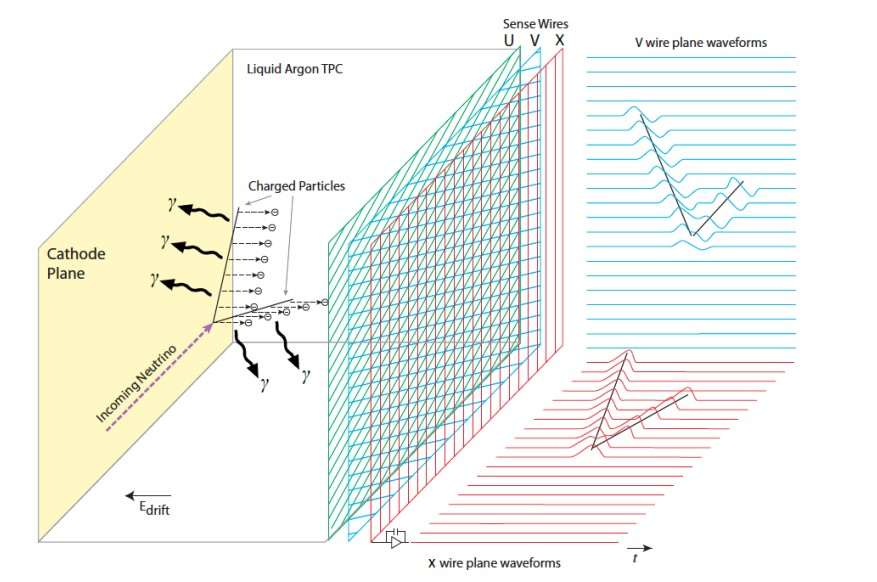
\includegraphics[width=\textwidth]{images/dune_tdrv12020_lartpc-sp.jpg}
\caption{Image of a Time Projection Chamber (TPC).
Charge is accumlated within the volume as ions are removed from the fidicial volume from another charged ion as it passes through the material.
An uniform electric field drifts the freed electrons towards the anode plane.
The collection and readout of charge on this anode plane is what is recorded within the detector.
Shown in the image are the three wire collection planes used in the DUNE experiment.
Image is taken from~\citep{DUNE_TDR_V1_Abi_2020}.}
\label{fig:dune_apa}
\end{figure}

The development of the TPC followed closedly with the devleopemnt of fast (> 1~\unit{MHz}) digitizing electronics.
With fast digitizers and closely spaced wires Georges Charpak (1924-2010) created the first multi-wire proportional chamber (MWPC) in 1968~\citep{Charpak:1968kd}.
Current and future TPCs~(see Section~\ref{sec:dune}) use MWPC as a basis for their readout electronics.

TPCs have been shown to be extremely capable in high energy physics experiments.
They are used in many applications such as dark matter experiments~\citep{Aprile_2017_xenon1T} and neutrino experiments~\citep{MicroBooNE_Acciarri_2017}.
TPCs are so useful because provide high resolution in both timing and spatial dimensions, as well as offer 3-D track reconstruction.
An example of the energy resolution and particle-identification capabilities of TPCs is shown in Figure~\ref{fig:pep4_tpc_dedex}.

\begin{figure}[]
\centering
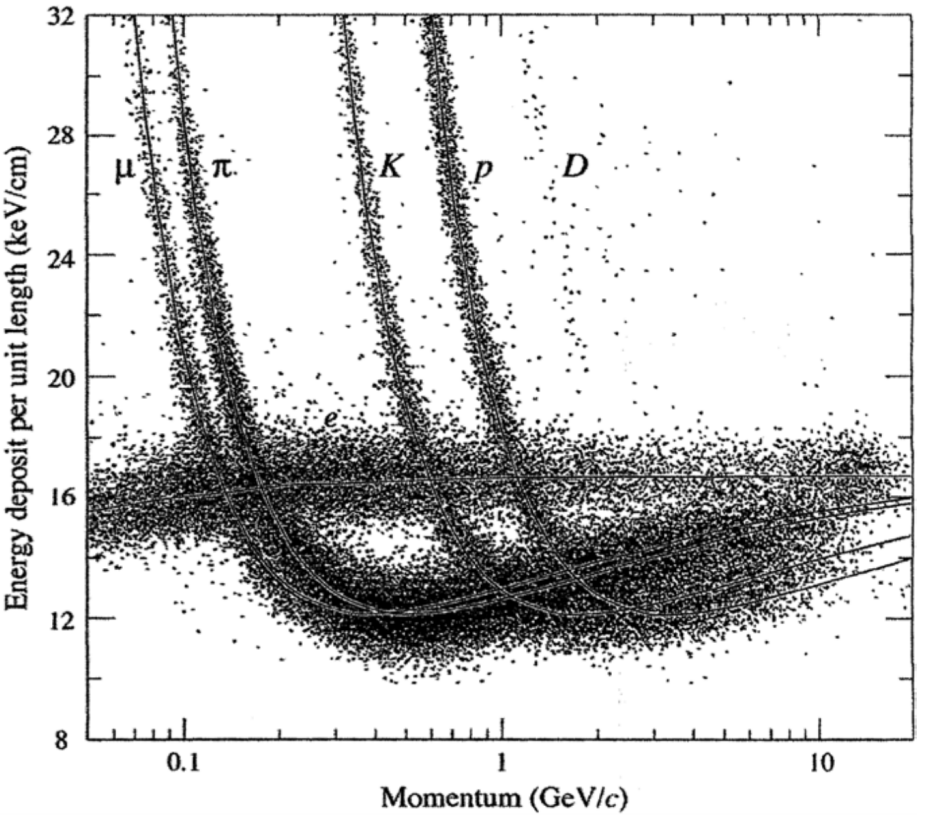
\includegraphics[width=0.8\textwidth]{images/pep4_tpc_dEdx.png}
\caption{Measurements of energy deposited in the PEP-4 detector.
These measurements show particle identification (PID) based on $\frac{dE}{dX}$.
The energy resolution for the PEP-4 experiment calculated to be 3\%.
Image taken from~\citep{pep_image}.
}
\label{fig:pep4_tpc_dedex}
\end{figure}


\subsection{Liquid Argon Time Projection Chambers}~\label{sec:lartpcs}

Alternatives to gaseous TPCs are liquid TPCs, which (as the name suggests) uses a liquid detection medium.
A specific kind of liquid based TCP is a Liquid Argon Time Projection Chamber (LArTPC)~\citep{rubbia1977liquid}.
Liquid was originally suggested as an alternative to the gaseous TPCs to provide a denser active volume.
Experiements such as neutrino or dark matter measurements have low interaction cross sections, and thus greatly benefit from a dense active detector medium.
Recently, much progress has been made in the implementation of LArTPCs for neutrino experiments (\citep{ArgoNeuT_PhysRevD.99.012002, MicroBooNE_Acciarri_2017, LArIAT_Acciarri_2020}).

LArTPCs provide a stable noble element (argon) which has high nucleon density.
Argon offers several key advantages for its selection as a detector medium.
Some key advantages of argon are its ability to produce large ($\sim$ 10kT) detectors, its high breakdown voltage, and its high ionization and scintillation yields.
The relevant properties of a LArTPC are shown in Table~\ref{tab:lar_prop}.

%% LAr table
\begin{table}
  \begin{center}
    \begin{tabular}{||c c c c||}
 \hline
      Property & Symbol & Value & Unit \\
 \hline\hline
      Density & $\rho$ &  1.3973 & $g cm^{-3}$ \\
      Dielectric Constant & $\epsilon$ & 1.505 & - \\
      electron drift velocity & $v_{e}$ & 0.1601 & $\unit{cm/\mu s}$ \\
      Ionization Energy of single $e^{-}$ & $W_{i}$ & 23.6 & eV/$e^{-}$ \\
      Minimum Specific energy loss & $(dE/dX)_{MIP}$ & 2.12 & MeV/cm \\
      Longitudinal Diffusion Coeffecients & $D_{L}$ & 6.6270 & $cm^{2}/s$ \\
      Transverse Diffusion Coeffecients & $D_{T}$ & 13.2327 & $cm^{2}/s$ \\
 \hline
    \end{tabular}
    \caption{
      Relevant Liquid Argon parameter information.
      Values are taken from~\citep{lardata_lbnl}, with temperature $T_{s} = 87 K$ and electric field $E_{f} = 0.5 kV cm^{-1}$.}
  \label{tab:lar_prop}
  \end{center}
\end{table}

\section{The Deep Underground Neutrino Experiment}~\label{sec:dune}

The Deep Underground Neutrino Experiment (DUNE) is a long-baseline neutrino beam experiment~\citep{DUNE_TDR_V1_Abi_2020, DUNE_FD_TDRv2_2020, DUNE_TDRv3_Abi_2020, DUNE-FD_TDRv4:Abi_2020}.
DUNE, when constructed, will be composed two detectors, a near detector (ND) and a far detector (FD) which are separated by a distance of 1300 km.
The neutrino beam measured at the ND and FD is generated in the Long Baseline Neutrino Facility (LBNF)~\citep{dune_cdr_2016_arxiv} beamline at Fermilab.
An image of the beam and the ND are shown in Figure~\ref{fig:dune_nd_beamline}.

The ND is located at Fermilab and its purpose is to characterize the unoscillated neutrino beam.
The ND serves as the DUNE's control.
Results from the interaction rates at the ND provide evidence for the null hypothesis within the standard three neutrino oscillation paradigm.
It will measure the unoscillated spectra for $\nu_{e}, \nu_{\mu}$, and their anti-particle pairs as a function of their energy, upon which the oscillation probability depends.
The FD will use these unoscillated measurements of the neutrino spectra to predict what neutrino interaction spectra it should measure.

\begin{figure}[]
\centering
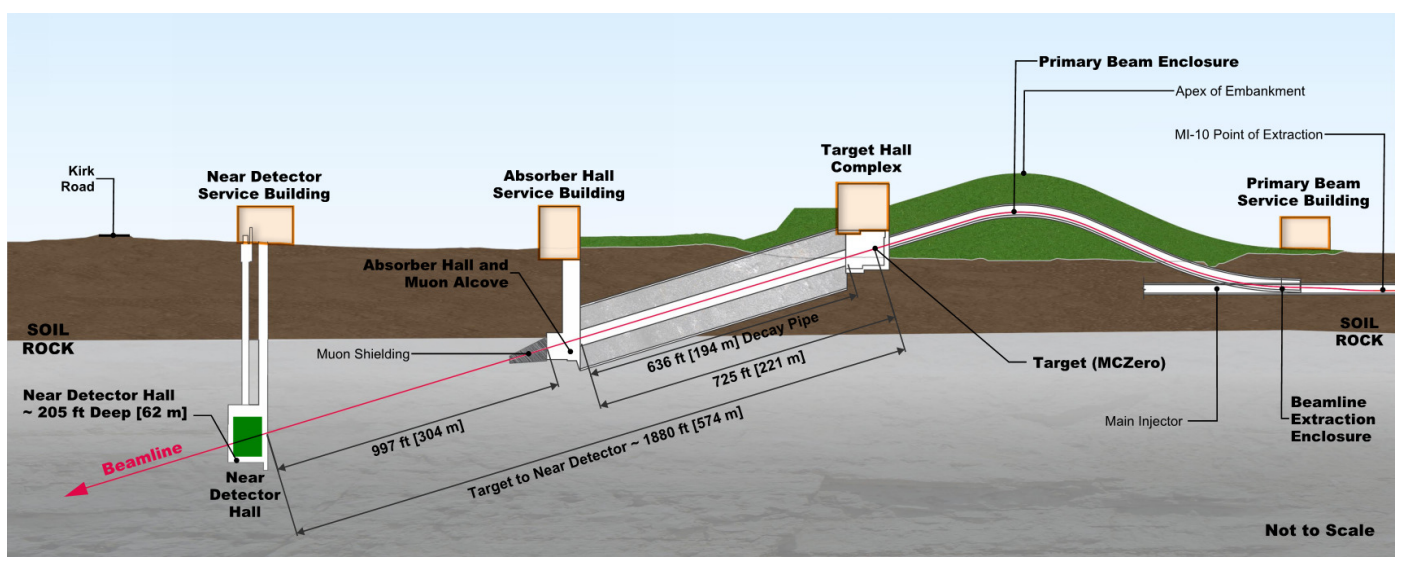
\includegraphics[width=\textwidth]{images/dune_nd_beamline_tdrv1.png}
\caption{Image of the near detector hall located relative to the neutrino beam at Fermilab in Illinois.
The ND is $\approx 525~\unit{m}$ from the neutrino target.
Image is taken directly from~\citep{DUNE_TDR_V1_Abi_2020}.
}
\label{fig:dune_nd_beamline}
\end{figure}


The ND is a suite of three detectors all exposed to a LBNF beam.
One component of the ND is a LArTPc (ND-LAr) which is a pixelated detector to be built using ArgonCube technology.
Another component of the ND is a high pressure (10~\unit{atm}) argon gas based TPC (ND-GAr).
The ND-Gar has superior identification abilities of charged pions than the LArTPC, and prevents misidentification of these pions as protons.
The final component of the ND is the System for on-Axis Neutrino Detection (SAND), which is a magnetized beam monitor.
SAND is used to measure the beam flux sent to the FD.

\begin{figure}[]
\centering
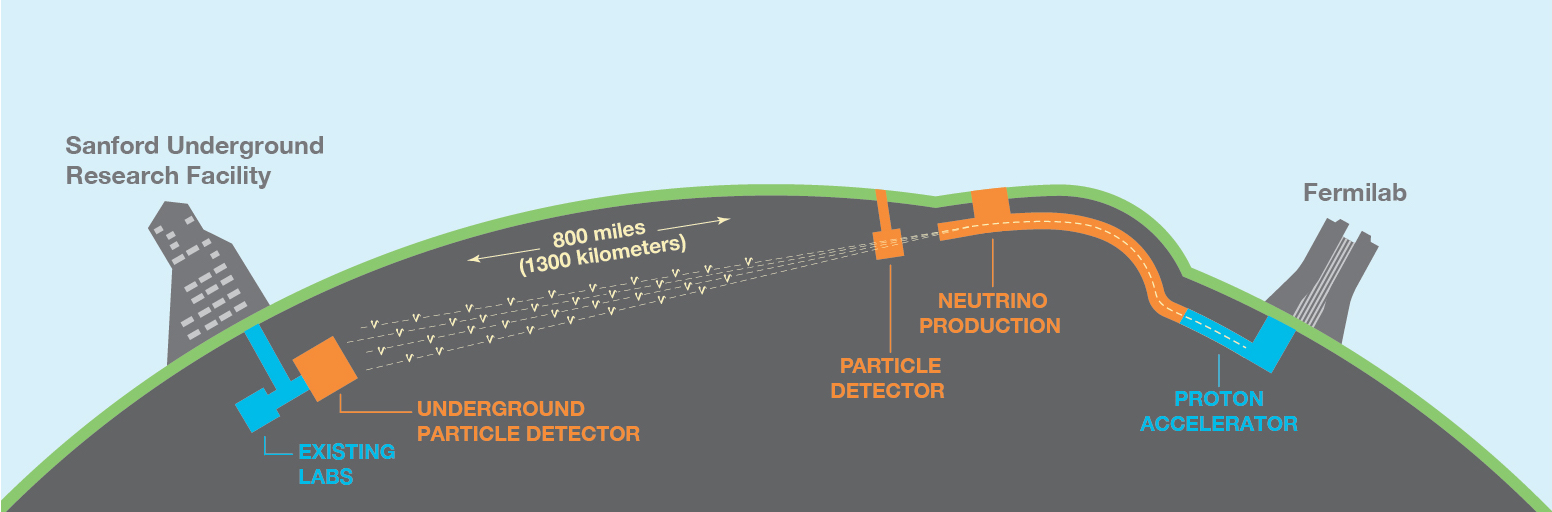
\includegraphics[width=\textwidth]{images/LBNE_Graphic_061615_2016.jpg}
\caption{Representation of the Near and Far Detectors for the DUNE experiment.
The ND is located within the image labeled as the Particle Detector.
One of the key purposes for the ND is to tag outgoing particles from the proton beam.
The FD is located at SURF on the left of the image, and will contain four 10 kT LArTPCs, which are the target of the neutrino beam.
The beam's energy and distance between the ND and FD are chosen to optimize sensitivity to neutrino oscillation measurements (See Section~\ref{sec:neutrino_oscillation}).
Image was taken from~\citep{dune_cdr_2016_arxiv}.}
\label{fig:dune_fd_image}
\end{figure}


The FD will be placed underground at Sanford Underground Research Facility (SURF) and be approximately 1300 km away from the ND.
The FD will be composed of four separate 10 kiloton LArTPC modules (DUNE-FD SP), an example of one is shown in Figure~\ref{fig:dune_10kt}.
This detector represents an enormous engineering challenge to place such a large, cold, and complicated detector.

At least two of these four modules at least will use a known wire-based readout technology.
The two remaining modules are considered modules of opportunity and their readout technology is yet unknown.
A purpose of this dissertation is show the viability of a novel readout technology targeted at a large 10~\unit{kT} LArTPC Single-Phase (SP) module, which is discussed in Chapter~\ref{chap:qpix}.

\begin{figure}[]
\centering
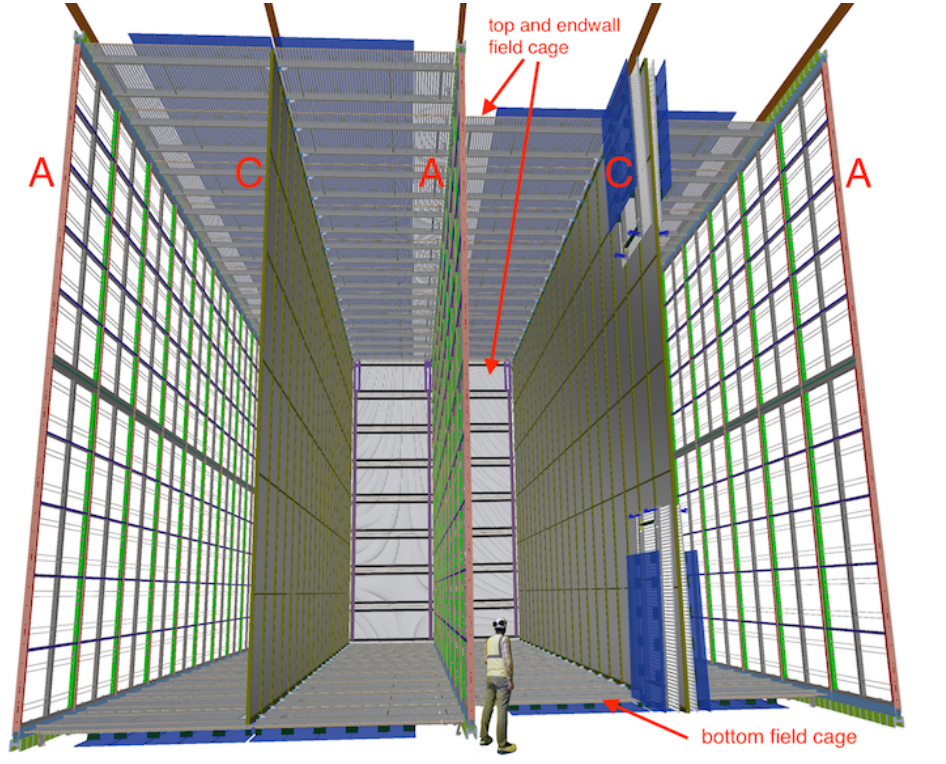
\includegraphics[width=\textwidth]{images/dune_fd_10ktmodule_tdrv1.png}
\caption{Image of a single 10~\unit{kT} DUNE Far-detector Single-Phase (DUNE-FD SP) module.
The dimensions of the module are 58.2~\unit{m} into the page, 12.0~\unit{m} high, and each drift distance is 3.5~\unit{m} between the anode (A) and cathode (C) planes. 
The ionization charges drift horrintally in the SP scheme, where electrons are drifted toward the anode (A) planes.
Image is taken directly from~\citep{DUNE_TDR_V1_Abi_2020}.
}
\label{fig:dune_10kt}
\end{figure}


DUNE has three main science goals, all of which are geared towards pushing beyond the SM:

\begin{itemize}
    \item Hadron Decay (Section~\ref{sec:hadron_decay})
    \item Core-collapse Supernovae (Section~\ref{sec:intro_supernova})
    \item Neutrino Oscillation (Section~\ref{sec:neutrino_oscillation})
\label{item:dune_props}
\end{itemize}

DUNE plans to offer an incredibly rich searches across the sectors listed above~\ref{item:dune_props}.
We will discuss the relevance of each of the first items in the next two sections.
We provide a more complete discussion of neutrino oscillations in Section~\ref{sec:neutrino_oscillation} because of its relevance to the results presented in Chapter~\ref{chap:sim}.


\subsection{Hadron Decay}~\label{sec:hadron_decay}

Does a proton decay?
This is the fundamental question for physicists studying hadron decay.
The SM predicts that the proton itself is stable, so it should never decay.
Therefore, the search for proton decays offers a path for physics beyond the SM.
Attempts to unify all the fundamental forces of nature into a unified theory are called Grand Unified Theories (GUTs), and according to many GUTs, the proton does indeed decay.

Current measurements on the proton lifetime indicate that its lifetime is on the order of magnitude (or above) $10^{34}$ years.
Even at its most frequent, this is an exceedingly rare event considering that the lifetime of the universe is $\approx \mathcal{O}(10^{10} yrs)$
Since these events are so rare, extremely large detectors with large numbers of protons inside of them are required to constantly observe many protons.
LArTPCs (like in DUNE) are excellent canidates to observe these rate events due to their active detector volume.
An example of a second generation proton decay studies is the Imaging Cosmic and Rare Underground Signals(ICARUS) experiment~\citep{ICARUS_2001}.

There are at least two prominant decay chains that are expected to be dominant, depending on the Grand-Unification-Theory (GUT) that hopes to go beyond the SM.
The first one is:
\begin{equation}~\label{eq:rxn_proton_decay1}
  p^{+} \rightarrow e^{+} + \pi^{0} + 2 \gamma
\end{equation}


This interaction is easily detectable in cherenkov based detectors due to the emission of both the gammas as well as the high energy of the emitted positron.
In fact, the worlds best estimate for proton lifetime comes from this decay-chain~\citep{PhysRevD.95.012004}.

Other Supersymmetric GUT models predict instead~\citep{PhysRevD.38.1479}:
\begin{equation}~\label{eq:rxn_proton_decay2}
  p^{+} \rightarrow K^{+} + \nu
\end{equation}

In this case the Kaon is generally moving too slow to be measurable by cherenkov detectors.
However, a TPC style detectors are still sensitive to its signature charge deposition.
This is an interesting reaction since the worlds best limits are currently provided by the Super-Kamiokande experiment, which is itself a cherenkov based detector in water.

These searches are interesting, if albeit difficult, both due to the rareness of such an event.
If any detector was able to clearly measure even a single proton decay, that would provide direct evidence for physics beyond the SM.
Future detectors that will continue to probe for nucleon decay are DUNE, Hyper-Kamiokande, and JUNO~\citep{DUNE_TDR_V1_Abi_2020, https://doi.org/10.48550/arxiv.1805.04163, Juno:2022103927}.

\subsection{Supernova Studies}~\label{sec:intro_supernova}

A supernova occurs when a massive star runs out of the necessary elemental fuel for fusion at its core.
When this happens the inward pull of gravity due to the mass of the star overcomes the reduced outward pressure from the nuclear fusion.

It has been nearly 30 years since the last observed neutrinos from a galactic core collapse supernova, SN 1987A~\citep{1987ApJ...322..795F}.
The rareness of these events encourage large, precise, long-running detectors to ensure a capture neutrinos from the next event.
Sensitivity to supernova neutrinos is crucial for understanding the mechanisms that govern particles at these extreme densities and pressures.
Interestingly, because neutrinos are so weakly interacting, it is possible to observe their signature and arrival before the photons arrival of a Type-II supernova.

The principal interaction chain observable in a TPC is:
\begin{equation}
    \nu_{e} + ^{40}Ar \rightarrow e^- + ^{40}Kr^{+}
\end{equation}

A LArTPC is sensitive to $\nu_{e}$ by measuring the signture of both the $e^{-}$ and $^{40}Kr^{+}$.
These events, when they occur happen within a small window of time (< 10~\unit{s}).
The first time interval of the SNB event is referred to as the neutrinization, which is primarily composed of $\nu_{e}$.
Therefore, any detector which expects to measure these events need to have either an constantly active and accurate trigger to detect these $\nu_{e}$ events, or continually record data.

\section{Neutrinos and Oscillations}~\label{sec:neutrino_oscillation}

Hints at the existence of neutrinos began early in the 20th century.
More than 100 years ago Chadwick was able to show that the energy spectrum from a decaying electron was continuous~\citep{Chadwick:1914zz}.
This unknown cause of the spectrum even lead some physicists to belief that perhaps the conservation of energy was violated.
Wolfgang Pauli instead predicted a particle which he originally called the neutron to also be a decay product, but not easily observable.
This third particle in the decay would explain the energy spectrum of the electron.
The discovery of the neutron(\citep{Chadwick1932PossibleEO}) and the continuous spectrum of beta decay forced Pauli to come up with a new theory attempting to describe beta decay~\citep{pauli_1934}.
finally, some 26 years later in 1956 the first observation of $\nu_{e}$~\citep{first_neutrino_measurement} was made.

Originally the mass of the neutrino predicted by the SM was massless.
That was until the Solar neutrino anomaly measured significantly less neutrinos than predicted~\citep{solar_neutrino_problem_PhysRevLett.20.1205}.
The solution for this was oscillation.
Since then, many large scale experiments have been dedicated to measuring the three generations of neutrinos.
~\citep{SNO_2002_neutrino_PhysRevLett.89.011301,
neutrino_measurement_NOvA_2019_prl,
t2k_2011_neutrino_PhysRevLett.107.041801,
reno_2012_neutrino_PhysRevLett.108.191802,
FUKUDA2002_solar_neutrino_oscillation,
kamland_2003_neutrino_PhysRevLett.90.021802,
daya_bay_2012_neutrino_PhysRevLett.108.171803,
PhysRevD.91.072010_t2k_2015,
doubleChooz_2012_neutrino_PhysRevLett.108.131801}
% Super-K / SNO / KamLand / NOvA / daya bay / RENO / double chooz / t2k / minos

Oscillation occurs because the mass eigenstate and flavor eigenstates are not equal.
Here we provide a general description of a model to describing neutrino oscillation.
We elucidate the measureable parameters which govern this oscillation and describe how these values are currently measured in experiments today.
The standard notation relates the mass eigenstates ($v_{i}$) and flavor eigenstates ($v_{\alpha}$):

Neutrino oscilLation is occurs to a neutrino as it moves through space can change its state.
\begin{equation}~\label{eq:relate_eigenstates}
  v_{i} = U_{i\alpha}v_{\alpha}
\end{equation}

% With adjoint of the matrix $U_{i\alpha}$, $U_{i\alpha}\dag$, we can then rewrite the equation:
% \begin{equation}
%   v_{\alpha} = U_{i\alpha}^{\dag}v_{i}
% \end{equation}
% \label{eq:adjoint_eigenstates}

%% neutrino mass oscillations
\begin{equation}~\label{eq:mass_eigenstates}
\begin{pmatrix}
\nu_e\\
\nu_{\mu}\\
\nu_{\tau}
\end{pmatrix}
=
\begin{pmatrix}
U_{e1}, U_{e2}, U_{e3} \\
U_{u1}, U_{u2}, U_{u3} \\
U_{\tau1}, U_{\tau2}, U_{\tau3}
\end{pmatrix}
\begin{pmatrix}
\nu_1\\
\nu_2\\
\nu_3
\end{pmatrix}
\end{equation}

The matrix elements within $U_{li}$ represent the mixing coeffecients and are used to calculate the prabability that a certain neutrino will oscillate from one family to another.
We identify $U_{ij}$ as the commonly known $U_{PMNS}$ matrix, where PMNS stands for: Pontecorvo–Maki–Nakagawa–Sakata, or the four theorists who helped developed this convention.
Luckily, there are not a total of nine free parameters within the SM that determine this.
The $U_{PMNS}$ matrix can be additionally rewritten following~\citep{Pontecorvo:1957qd, 1962PThPh..28..870M} as:

\begin{equation}~\label{eq:uij_matrix_simp}
U_{PMNS}
=
U_{sol} \times U_{rea} \times U_{atm} \times U_{maj}
\end{equation}

After expanding the matrix representations, equation~\ref{eq:uij_matrix_simp} becomes:
\begin{equation}
U_{PMNS}
=
\begin{pmatrix}
1 & 0 & 0 \\
0 & C_{23} & S_{23} \\
0 & -S_{23} & C_{23} \\
\end{pmatrix}
\times
\begin{pmatrix}
C_{13} & 0 & S_{13}e^{-1\delta_{cp}} \\
0 & 1 & 0 \\
-S_{13}e^{-1\delta_{cp}} & 0 & C_{13} \\
\end{pmatrix}
\times
\begin{pmatrix}
C_{12} & S_{12} & 0 \\
-S_{12} & C_{12} & 0 \\
0 & 0 & 1 \\
\end{pmatrix}
\times
\begin{pmatrix}
0 & 0 & 1 \\
e^{i\alpha_{1}} & 0 & 0 \\
0 & e^{i\alpha_{2}} & 0 \\
\end{pmatrix}
\end{equation}

We identify above the additional matrix components where historically these values are measured.
Therefore, instead of nine unknown parameters for the SM, there are only six.
The components $C_{ij}$ and $S_{ij}$ in the matrices are defined to be $\cos(\theta_{ij})$ and $\sin(\theta_{ij})$, respectively.

Then, the six parameters of the $U_{PMNS}$ are identified as:
\begin{itemize}
    \item $\theta_{13}$ - Reactor measurements.
    \item $\theta_{12}$ - Atmospheric measurements.
    \item $\theta_{23}$ - Solar measurements.
    \item $\delta_{CP}$ - Charge-conjugation parity violation.
    \item $\alpha_{1}$/$\alpha_{2}$, The two Majorana Phase parameters, not observable in beam experiments.
\end{itemize}

The Majorana phases ($\alpha_{i}$) are sensitive in experiments that can detect the Majorana nature of neutrions such as neutrinoless double beta decay.
In neutrino oscillation measurements, these phases cancel out and not not measureable.
Therefore, we can safely ignore these two phases for the work presented here.

Next we demonstrate the calculation of the probability of oscillation from one mass eigenstate to another.
Namely we calculate the probablity $P(\mu \rightarrow e)$ which is the probability of interest in a long beamline experiment.
First we identify that equation~\ref{eq:relate_eigenstates} can be rewritten to isolate the flavor-eigenstate terms ($v_{\alpha}$) by multiplying by the adjoint of the PMNS matrix ($U^{*}_{PMNS}$).
Then the relationship between the time dependent mass and flavor eigenstates become:

\begin{equation}~\label{eq:flavor_relation}
\ket{v_{\alpha}(t)} = U^{*}_{PMNS}\ket{v_{i}(t)}
\end{equation}

The value of interest is $P(\mu \rightarrow e)$, which occurs if the $\nu_{\mu}$ travels after some time, t, and interacts via a charged-current (CC) interaction.
The probability to end up in state $v_{e}$ beginning from $v_{\mu}$ is:

\begin{equation}~\label{eq:prob_calc1}
P(\mu \rightarrow e) = \lvert \braket{ v_{e} | v_{\mu} (t) }\rvert^{2}
\end{equation}

We then use equation~\ref{eq:flavor_relation} to represent the matrix elements of $U_{PMNS}$ from $v_{e}$ and $v_{\mu}$  to obtain:
\begin{equation}~\label{eq:prob_calc2}
  P(\mu \rightarrow e)
  = \lvert \sum_{i} U_{e i} U^{*}_{\mu i} e^{-i E_{i}t} \rvert^{2} \\
  =
  \delta_{ij}
  - 4 \sum_{i>j}  \Re( U^{*}_{ej}U_{\mu j}U_{ei}U^{*}_{\mu i} ) \sin ^2(\frac{m_{ij}^{2}}{4E}L)
  + 2 \sum_{i>j}  \Im( U^{*}_{ej}U_{\mu j}U_{ei}U^{*}_{\mu i} ) \sin(\frac{m_{ij}^{2}}{2E}L)
\end{equation}

Where we identify that the cross terms introduce a phase difference shown as $\Delta_{ij}$ in the second term in Equation~\ref{eq:prob_calc2}.
This represents the neutrino oscillation term and represents the difference in the mass states of the neutrinos:
\begin{equation}
\Delta_{ij} = (E_{i} - E_{j})
\end{equation}

The energy of the neutrino in each state can be approximated to first order following:

\begin{equation}
E_{i} = \sqrt{p^2 + m_{i}^{2}} \approx p + \frac{m^{2}_{i}}{2p}
\end{equation}

Since the momentumum of all of the mass eigenstates is the constant.
Then oscillation parameter becomes:
\begin{equation}
\Delta_{ij} \approx \frac{1}{2p}(m^2_{i}-m^{2}_{j}) = \frac{\Delta m_{ij}^2}{2p}
\end{equation}

Finally, the last two parameters which govern the neutrino oscillations are identified as the mass differences between the three mass states.
These two mass-squared differences are represented in Figure~\ref{fig:mass_hierarchy}.
Unfortunately, the the sign of $m_{13}$ is unknown.
This leads to two possible orderings of the masses, known as normal (NO) and inverted (IO) order.
NO indicates that the masses of the neutrinos follow the ordering of their charged partners.
That is, NO implies a mass ordering of: $\nu_{e} < \nu_{\mu} < \nu_{\tau}$.
Whereas, IO has a mass ordering: $\nu_{\tau} < \nu_{e} < \nu_{\mu}$.

\begin{figure}[]
\centering
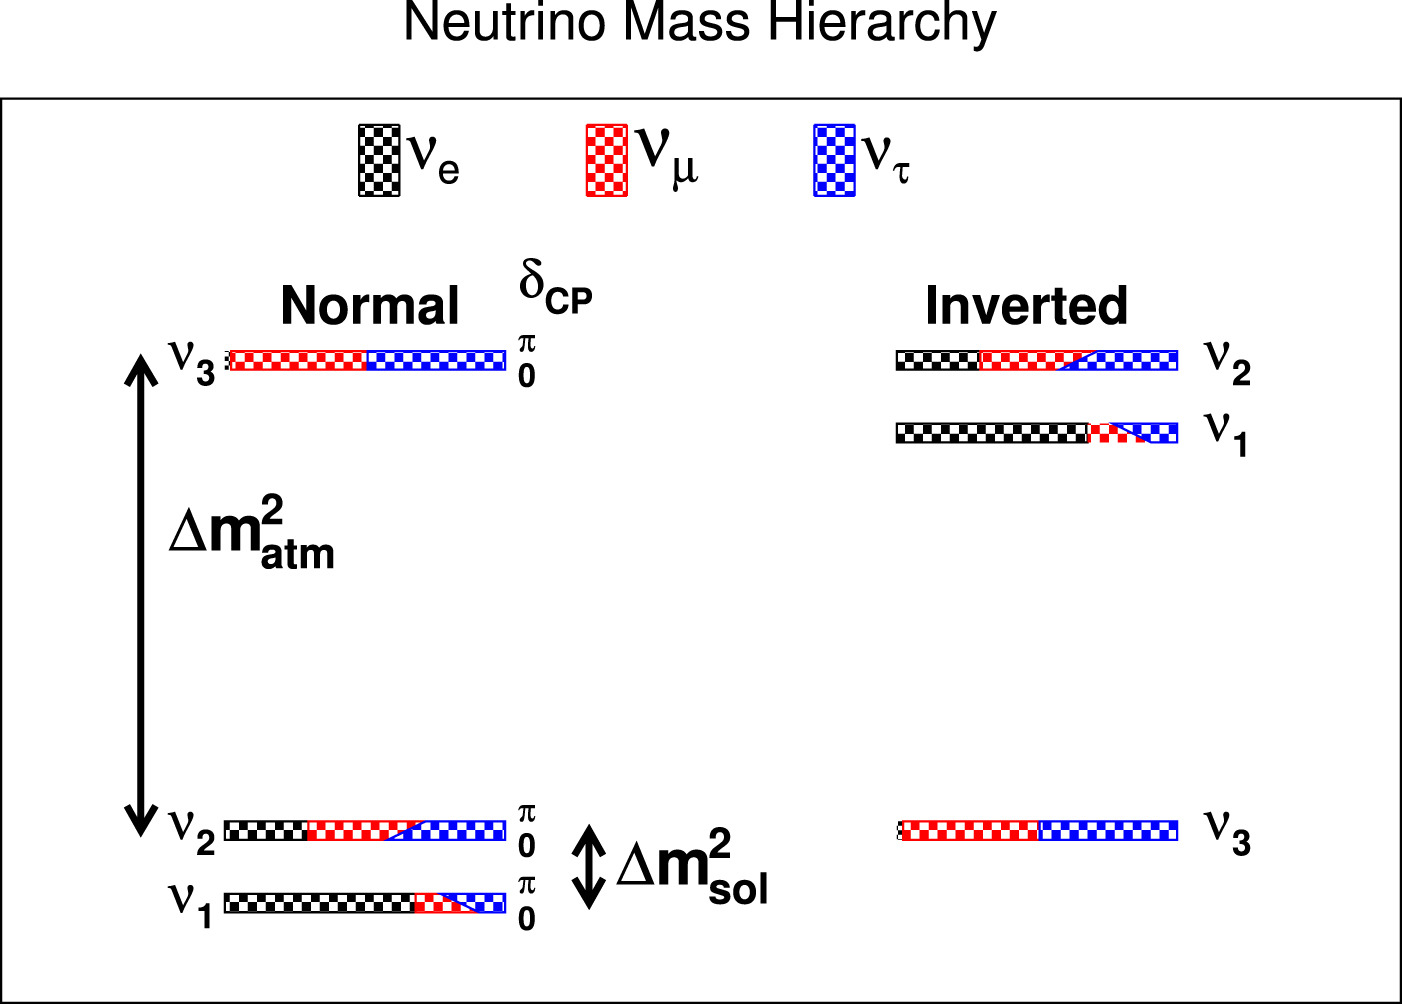
\includegraphics[width=\textwidth]{images/mass_hierarchy.jpg}
\caption{Representation of the mass hierarchy scales. This is a represntation of the two possible orderings of neutrino massses, due to the uncertain sign of $m_{13}$. It is also interesting to observe that the absolute mass scale is not measured since oscillation measurements only give difference mass squares. Image was taken from~\citep{QIAN20151}.}
\label{fig:mass_hierarchy}
\end{figure}

Neutrino oscillations in matter are slightly different than those in vacuum~\citep{PhysRevD.17.2369}.
The Mikheyev-Smirnov-Wolfenstein (MSW) effect~\citep{Smirnov2004TheME} also contributes to differening neutrino oscillations as they move through matter of varying density, which additionally complicated the calculation.
The MSW effect also affects neutrinos differently than anti-neutrinos, which is useful for measuring $\delta_{cp}$.
This resonance effect for beam-line experiments affects $\nu_{e}$ in the case of normal mass ordering (NO), whereas in the case of inverted mass order (IO), the $\hat{\nu_{e}}$ experiences resonance and is thus more likely.

\begin{table}
\begin{center}
\begin{tabular}{||c c c c||}
 \hline
 Paramater & Best Fit & Unit & Best Soruce\\ [0.5ex]
 \hline\hline
  $\theta_{13}$ & $8.57^{+0.12}_{-0.12}$ & na & Reactor \\ % DAYA/doubleChooz/RENO 2012 Daya Bay found not equal to zero
 \hline
  $\theta_{12}$ & $33.44^{+0.77}_{-0.74}$ & na & Atmospheric \\ % KamLAND + SNO, liquid scintillator
 \hline
  $\theta_{23}$ & $49.2^{+0.9}_{-1.2}$ & na & Solar \\ % Solar, T2k(water cherenkov) / NOvA(liquid scintillator / numi off axis)
 \hline
  $\delta_{cp}$ & $197^{+27}_{-24}$ & na & Atmospheric+Accelerator \\ % t2k / NOva, https://pdg.lbl.gov/2022/listings/rpp2022-list-neutrino-mixing.pdf
 \hline
  $\Delta m_{21}^{2}$ & $7.42^{0.21}_{-0.20}$ & $10^{-5}eV^{2}$ & Solar \\ % kamland / SNO / SKAM
 \hline
  $\Delta m_{3l}^{2}$ & $2.517^{+0.026}_{-0.028}$ & $10^{-3}eV^{2}$ & Atmospheric  \\
 \hline
\end{tabular}
\caption{Known Oscillation Parameters of Interest.
Values are taken from the global fit~\citep{2020JHEP...09..178E}.
The values shown assume normal mass ordering for neutrinos and include atmospheric Super-Kamikonde Data.
}
\end{center}
\end{table}~\label{table:pmns_params}

\section{Towards Future Detectors}~\label{sec:future_detectors}

%% antihydrogen
\citep{Sadowski_2017}
Another driving factor is the the development of Machine Learning (ML) algorithms, particularly Convectional Neural Network (CNN \citep{Sadowski2017DeepLI}).
Recent industry has driven the need for CNNs to be able to correctly identify and label 2-D images of various kinds, and thus championed much of progress in this field and spawned many kinds of CNN algorithms.

%% cite sadowski here
Recently, it has been shown how these kinds of algorithms extend into High Energy Physics (HEP) for particle identification.
A major issue at the Intensity Frontier of physics is the sheer amount of data to store and process.
These ML algorithms provied a developed tool to automate the analysis of huge amounts of data ($>> 1 TB$) and have been shown to be quite accurate ($>99\%$) at particle identification in LArTPCs.


%% LArPix / Argon Cube
Additional work has been performed in recent years which show that LArTPCs can also utilized a pixel-based readout~\citep{larpix:Dwyer_2018}, \citep{Asaadi_2018}.

The end of the Standard Model era is inevitable.
SM simply fails to account for physics with all major frontiers for physicists to accept its completeness; we know there is much and more to learn about nature.

The 20th century saw unprecedented progress in its sophistication of its detectors from ray tubes, to spark chambers, to proportional counters, and to huge (>20 km) particle accelerators.
This century shows no signs holding any less promise than its predecessor.
Continued development in electronics, computing, and analysis methods will lead to more and newer frontiers of physics.

The work presented in this introduction aims to not only encapsulate the massive progress particle physics has made since the electron's discovery, but also to server as a reminder of how extraordinarily surprising nature is.
At every turn and at every point where physicists think they've arrived at the end (or at an impossible roadblock) there always remains more to discover.
If we have learned anything, we have learned to knock and the door shall be opened.

% \begin{table}
% \begin{center}
% \begin{tabular}{||c c c c c||}
%  \hline
%  Lepton & Charge & $N_{e}$ & $N_{\mu}$ & $N_{\tau}$ \\ [0.5ex]
%  \hline\hline
%  $e^{-}$ & 1 & 1 & 0 & 0 \\
%  \hline
%  $\nu_{e}$ & 0 & 1 & 0 & 0 \\
%  \hline
%  $\mu$ & 1 & 0 & 1 & 0 \\
%  \hline
%  $\nu_{\mu}$ & 0 & 0 & 1 & 0 \\
%  \hline
%  $\tau$ & 1 & 0 & 0 & 1 \\
%  \hline
%  $\nu_{\tau}$ & 0 & 0 & 0 & 1 \\
%  \hline
% \end{tabular}
% \caption{Description of the quantum numbers of the fundamental lepton families.
%   There are three unique families within the leptons: electron, muon, and tau.
%   The charge carrier as well as the neutrino each carry a value of one for this number.
%   Their anti-particle counterparts carry -1 of this number.}
% \end{center}
% \end{table}
% ~\label{table:lepton_qn}


More detailed descriptions of such collider experiments are beyond the scope of the work presented here, and further reading may be pursued from the extremely detailed technical design reports cited here of Belle-II and the ATLAS experiments.
The LHC itself consists of other large-scale tracking and calioremtry experiments such as ATLAS~\citep{ATLAS:1999vwa} and CMS~\citep{CMS:2006myw}.
There exist lepton collidors~\citep{belle2_tdr_arxiv} which offer unique areas of search along this frontier too.